\documentclass[12pt]{article}
\usepackage[utf8]{inputenc}
\usepackage{amsmath}
\usepackage{pgfplots}
\usepackage{tcolorbox}
\usepackage{graphicx}
\usepackage{booktabs}
\usepackage{geometry}
\usepackage{hyperref}
\usepackage{fancyhdr}
\usepackage{lastpage}

\geometry{a4paper, margin=1in}
\pagestyle{fancy}
\fancyhead[LO]{Jack Zeng}
\fancyhead[RO]{Page \thepage\ of \pageref{LastPage}}

\begin{document}

\section*{SAT Hard Question 4}
\begin{tcolorbox}[colback=green!10, colframe=green!50!black, title=Question 29: Probability (Statistics)]
\textbf{Handedness Table:}

\begin{center}
\begin{tabular}{|c|c|c|}
\hline
\textbf{Gender} & \textbf{Left} & \textbf{Right} \\
\hline
Female &  &  \\
\hline
Male &  &  \\
\hline
Total & 18 & 122 \\
\hline
\end{tabular}
\end{center}

The incomplete table above summarizes the number of left-handed students and right-handed students by gender for the eighth-grade students at Keisel Middle School. 

There are **5 times** as many right-handed female students as there are left-handed female students, and **9 times** as many right-handed male students as there are left-handed male students.

If there is a total of **18** left-handed students and **122** right-handed students in the school, which of the following is closest to the probability that a right-handed student selected at random is female?

**(Note: Assume that none of the eighth-grade students are both right-handed and left-handed.)**

\textbf{Answer Choices:}
\begin{itemize}
    \item \textbf{A.} \( 0.410 \) 
    \item \textbf{B.} \( 0.357 \)
    \item \textbf{C.} \( 0.333 \)
    \item \textbf{D.} \( 0.250 \)
\end{itemize}

\textbf{Correct Answer:} \( 0.41 \) (correct)

\textbf{Explanation:} 
Let \( x \) represent the number of left-handed females, and \( y \) represent the number of left-handed males.

Since the total number of left-handed students is 18:
\[
x + y = 18.
\]
Given the problem conditions:
\[
\text{Right-handed females} = 5x, \quad \text{Right-handed males} = 9y.
\]
The total right-handed students sum up to 122:
\[
5x + 9y = 122.
\]

\end{tcolorbox}

\begin{tcolorbox}[colback=green!10, colframe=green!50!black, title=Question 38: Little's Law (Problem Solving)]
\textbf{Questions 37 and 38 refer to the following information.}

If shoppers enter a store at an average rate of \( r \) shoppers per minute and each stays in the store for an average time of \( T \) minutes, the average number of shoppers in the store, \( N \), at any one time is given by the formula:
\[
N = rT.
\]
This relationship is known as \textbf{Little’s law}.

The owner of the Good Deals Store estimates that during business hours, an average of \( 3 \) shoppers per minute enter the store and that each of them stays an average of \( 15 \) minutes. The store owner uses Little’s law to estimate that there are \( 45 \) shoppers in the store at any time.

\vspace{5mm}
\textbf{Question 38:} 

The owner of the Good Deals Store opens a new store across town. For the new store, the owner estimates that, during business hours, an average of \( 90 \) shoppers per \textbf{hour} enter the store and that each of them stays an average of \( 12 \) minutes. The average number of shoppers in the new store at any time is what percent less than the average number of shoppers in the original store at any time?

\textbf{(Note: Ignore the percent symbol when entering your answer. For example, if the answer is 42.1\%, enter 42.1.)}

\textbf{Answer Choices:}
\begin{itemize}
    \item \( 57 \)
    \item \( 58 \)
    \item \( 59 \)
    \item \( 60 \) 
\end{itemize}

\textbf{Correct Answer:} \( 60 \) (Correct)

\textbf{Explanation:} 
For the original store:
\[
N = 3 \times 15 = 45.
\]
For the new store, converting \( 90 \) shoppers per hour to per minute:
\[
r = \frac{90}{60} = 1.5.
\]
Using Little's Law:
\[
N = 1.5 \times 12 = 18.
\]

Percentage decrease:
\[
\frac{45 - 18}{45} \times 100 = 60\%.
\]

Thus, the number of shoppers in the new store is \textbf{60\% less} than in the original store.
\end{tcolorbox}



\begin{tcolorbox}[colback=green!10, colframe=green!50!black, title=Question 2: Statistical Generalization]
A trivia tournament organizer wanted to study the relationship between the number of points a team scores in a trivia round and the number of hours that a team practices each week. 

For the study, the organizer selected **55** teams at random from all trivia teams in a certain tournament. The table displays the information for the **40** teams in the sample that practiced for at least **3 hours per week.**

\begin{center}
\begin{tabular}{|c|c|c|c|}
\hline
\textbf{Hours practiced} & \multicolumn{2}{c|}{\textbf{Number of points per round}} & \textbf{Total} \\
\hline
 & \textbf{6 to 13 points} & \textbf{14 or more points} &  \\
\hline
\textbf{3 to 5 hours} & 6 & 4 & 10 \\
\textbf{More than 5 hours} & 4 & 26 & 30 \\
\hline
\textbf{Total} & 10 & 30 & 40 \\
\hline
\end{tabular}
\end{center}

Which of the following is the **largest population** to which the results of the study can be generalized?

\textbf{Answer Choices:}
\begin{itemize}
    \item \textbf{A.} All trivia teams in the tournament that scored **14 or more points** in the round.
    \item \textbf{B.} The **55 trivia teams** in the sample.
    \item \textbf{C.} The **40 trivia teams** in the sample that practiced for at least **3 hours per week.**
    \item \textbf{D.} All trivia teams in the **tournament.**
\end{itemize}

\end{tcolorbox}

\begin{tcolorbox}[colback=green!10, colframe=green!50!black, title=Question 20: Tangent Line and Circle Geometry]
\textbf{Given:} 

The circle shown has center \( (-1,1) \). Line \( t \) is tangent to this circle at point \( (4,-3) \). 

\begin{center}
    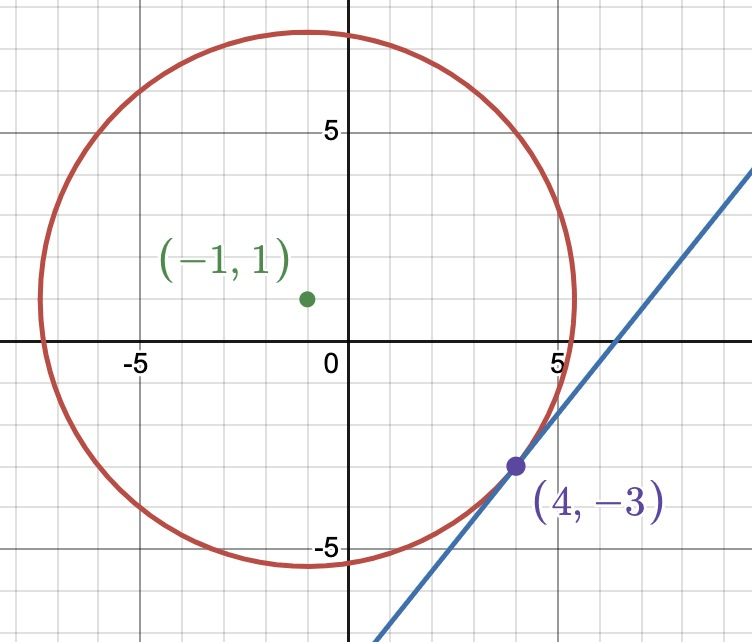
\includegraphics[width=0.5\linewidth]{f3.jpg}
\end{center}

Which of the following points lies on line \( t \)?

\textbf{Answer Choices:}
\begin{itemize}
    \item \textbf{A.} \( (0, \frac{5}{4}) \)
    \item \textbf{B.} \( (3,6) \)
    \item \textbf{C.} \( (8,2) \)
    \item \textbf{D.} \( (9,1) \)
\end{itemize}

\vspace{5mm}
\textbf{Final Answer:} The correct point on the tangent line is **\( (8,2) \), answer choice C.
\end{tcolorbox}


\newapage
\begin{tcolorbox}[colback=green!10, colframe=green!50!black, title=Question 10: Rectangular Prism Surface Area]
\textbf{Given:} 

Two identical rectangular prisms each have a height of **90 cm**. The base of each prism is a square, and the surface area of each prism is **\( K \) cm\(^2\)**.

If the prisms are glued together along a square base, the resulting prism has a surface area of:
\[
\frac{92}{47} K \text{ cm}^2.
\]

What is the side length, in cm, of each square base?


\vspace{5mm}
\textbf{\[
s = 8.
\]}
\end{tcolorbox}


\begin{tcolorbox}[colback=green!10, colframe=green!50!black, title=Question 12: Triangle Similarity and Area]
\textbf{Given:} 

In triangle \( RST \), angle \( T \) is a right angle. Point \( L \) lies on \( \overline{RS} \), point \( K \) lies on \( \overline{ST} \), and \( \overline{LK} \) is parallel to \( \overline{RT} \).

Given:
\begin{itemize}
    \item \( RT = 72 \) units,
    \item \( LK = 24 \) units,
    \item Area of \( \triangle RST = 792 \) square units.
\end{itemize}

Find the length of \( KT \), in units.


\end{tcolorbox}
\newpage
\begin{tcolorbox}[colback=green!10, colframe=green!50!black,title=Question 3: Circle Equation (Geometry)]
Given the circle equation \( (x - 6)^2 + (y + 5)^2 = 16 \) and point \( P(10, -5) \) on the circle, where \( PQ \) is the diameter:
\begin{itemize}
    \item What are the coordinates of point \( Q \)?
\end{itemize}
\end{tcolorbox}







\end{document}